% Created 2021-03-15 Mon 21:14
% Intended LaTeX compiler: pdflatex
\documentclass[presentation]{beamer}
\usepackage[utf8]{inputenc}
\usepackage[T1]{fontenc}
\usepackage{graphicx}
\usepackage{grffile}
\usepackage{longtable}
\usepackage{wrapfig}
\usepackage{rotating}
\usepackage[normalem]{ulem}
\usepackage{amsmath}
\usepackage{textcomp}
\usepackage{amssymb}
\usepackage{capt-of}
\usepackage{hyperref}
\usepackage{minted}
\usepackage[utf8]{inputenc}
\usepackage{color}
\usetheme[height=7mm]{Rochester}
\setbeamertemplate{footline}[frame number]
\usecolortheme[accent=red, light]{solarized}
\setbeamercolor{frametitle}{bg=solarizedRebase02,fg=solarizedAccent}
\setbeamercolor{author in head/foot}{bg=solarizedRebase02,fg=solarizedRebase01}
\setbeamercolor{title in head/foot}{bg=solarizedRebase02,fg=solarizedRebase01}
\setbeamercolor{block title}{bg=solarizedRebase0,fg=solarizedRebase02}
\setbeamercolor{block body}{bg=solarizedRebase02,fg=solarizedRebase0}
\setbeamercolor{item}{bg=solarizedRebase02,fg=solarizedAccent}
\beamertemplatenavigationsymbolsempty
\usemintedstyle{manni}
\AtBeginSection[]{
\begin{frame}
\vfill
\centering
\begin{beamercolorbox}[sep=8pt,center,shadow=true,rounded=true]{title}
\Huge\insertsectionhead\par%
\end{beamercolorbox}
\vfill
\end{frame}
}
\usetheme{default}
\author{Sebastian Stabinger, Thomas Hausberger}
\date{SS2021}
\title{2D Arrays}
\hypersetup{
 pdfauthor={Sebastian Stabinger, Thomas Hausberger},
 pdftitle={2D Arrays},
 pdfkeywords={},
 pdfsubject={},
 pdfcreator={Emacs 27.1 (Org mode 9.4.4)}, 
 pdflang={Ger}}
\begin{document}

\maketitle
\section{2D Arrays im Speicher}
\label{sec:org086c82d}
\begin{frame}[label={sec:org3de9423}]{Das Problem mit 2D Arrays}
\begin{itemize}
\item Wir würden gerne 2D Arrays (z.B. Matrizen) in C verwenden.
\item Das Problem: \alert{Speicher ist} üblicherweise (bis auf sehr seltene
Spezialhardware) \alert{eindimensional}
\item Wir müssen also eine Möglichkeit finden um ein \alert{2D Array mit Hilfe
eines 1D Arrays zu simulieren}
\item Wir besprechen das Problem und die Lösung an Hand von 2D Arrays. Das
Problem und die Lösungen \alert{gelten aber genauso für alle
höherdimensionalen} Arrays (z.B. 3D Tensoren)
\end{itemize}
\end{frame}
\section{2D-Arrays in C implementiert?}
\label{sec:org97e47c1}
\begin{frame}[label={sec:org0373789}]{Zwei Möglichkeiten}
\begin{itemize}
\item In C integrierte mehrdimensionale Arrays
\item Manuelle Lösung
\end{itemize}
\end{frame}
\begin{frame}[label={sec:orgc50470e},fragile]{In C integrierte Version}
 \begin{block}{Syntax:}
{\color{solarizedYellow}\texttt{datentyp name[Zeilenanzahl][Spaltenanzahl];}}
\end{block}
\begin{block}{Beispiel}
\begin{minted}[fontsize=\scriptsize,numberblanklines=false]{c}
int a[3][4];
a[1][2] = 23;
a[0][3] = 42;
printf("Wert in Zeile 2, Spalte 3 = %d", a[1][2]);
\end{minted}
\end{block}
\begin{block}{Es sind auch mehr als zwei Dimensionen möglich}
\begin{minted}[fontsize=\scriptsize,numberblanklines=false]{c}
// 4D Array
double arr[12][34][42][3];
\end{minted}
\end{block}
\end{frame}
\begin{frame}[label={sec:org7877d90},fragile]{Visualisierung}
 Was passiert im Speicher bei {\color{solarizedYellow}\texttt{int a[3][4];}}?
\begin{itemize}
\item Man reserviert Speicher für ein \alert{Array mit 3 Elementen}, wobei
\alert{jedes Element ein Array mit vier Integer Werten} ist!
\end{itemize}
\begin{center}\begin{center}
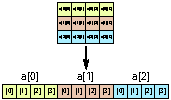
\includegraphics[width=0.8\textwidth]{2dto1d.pdf}
\end{center}\end{center}
\begin{itemize}
\item {\color{solarizedYellow}\texttt{a[1]} }liefert also z.B. das Array für die zweite Zeile des Arrays
zurück auf dessen drittes Elemente man dann mittels {\color{solarizedYellow}\texttt{[2]} }zugreift
\end{itemize}
\end{frame}
\begin{frame}[label={sec:org47c32d7},fragile]{Initialisieren}
 \begin{block}{Verschachtelte Initialisierungslisten}
\begin{minted}[fontsize=\scriptsize,numberblanklines=false]{c}
int a[3][4] = {{1, 2, 3, 4}, {5, 6, 7, 8}, {9, 10, 11, 12}};
\end{minted}
\end{block}
\begin{block}{Manuell}
\begin{minted}[fontsize=\scriptsize,numberblanklines=false]{c}
for (int r = 0; r < 3; r++)
  for (int c = 0; c < 4; c++)
    a[r][c] = 0;
\end{minted}
Achtung: Die innerste Schleife sollte ueber die letzte Dimension
iterieren, da dies schneller ist!
\end{block}
\end{frame}
\begin{frame}[label={sec:org5b85d90},fragile]{In C integrierte Version --- Beispiel}
 \begin{block}{Beispiel}
\begin{minted}[fontsize=\scriptsize,numberblanklines=false]{c}
#include <stdio.h>

int main() {
  int a[3][4] = {{1, 2, 3, 4}, {5, 6, 7, 8}, {9, 10, 11, 12}};

  for (int row = 0; row < 3; row++) {
    for (int col = 0; col < 4; col++)
      printf("%d\t", a[row][col]);
    printf("\n");
  }
}
\end{minted}
\end{block}
\end{frame}

\begin{frame}[label={sec:orgac48ce4}]{Übergabe an Funktionen}
Um auf Werte eines 2D Arrays zugreifen zu können, muss C wissen wie
viele Werte eine Zeile enthält!
\begin{center}\begin{center}
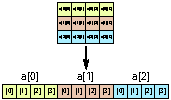
\includegraphics[width=0.5\textwidth]{2dto1d.pdf}
\end{center}\end{center} 

\(\rightarrow\) Wenn ein mehrdimensionales Array \alert{an eine Funktion
übergeben} wird muss die Größe aller Dimensionen bis auf die erste
\alert{bekannt} sein!
\end{frame}
\begin{frame}[label={sec:orgb4f8eca},fragile]{Übergabe an Funktionen --- Beispiel}
 \begin{block}{Beispiel}
\begin{minted}[fontsize=\scriptsize,numberblanklines=false]{c}
#include <stdio.h>

void print_matrix(int arr[][4], int rows) {
  for (int row = 0; row < rows; row++) {
    for (int col = 0; col < 4; col++)
      printf("%d\t", arr[row][col]);
    printf("\n");
  }
}

int main() {
  int a[3][4] = {{1, 2, 3, 4}, {5, 6, 7, 8}, {9, 10, 11, 12}};
  print_matrix(a, 3);
}
\end{minted}
\end{block}
\end{frame}

\begin{frame}[label={sec:orgc61af48},fragile]{Übergabe an Funktionen --- Beispiel seit C99}
 \begin{itemize}
\item Seit C99 können übergebene Parameter statt fixen Größen verwendet
werden
\end{itemize}
\begin{block}{Beispiel}
\begin{minted}[fontsize=\scriptsize,numberblanklines=false]{c}
#include <stdio.h>

void print_matrix(int rows, int cols, int arr[][cols]) {
  for (int row = 0; row < rows; row++) {
    for (int col = 0; col < cols; col++)
      printf("%d\t", arr[row][col]);
    printf("\n");
  }
}

int main() {
  int a[3][4] = {{1, 2, 3, 4}, {5, 6, 7, 8}, {9, 10, 11, 12}};
  print_matrix(3, 4, a);
}
\end{minted}
\end{block}
\end{frame}

\begin{frame}[label={sec:org5f55b82}]{Manuell}
\begin{itemize}
\item Das was C intern macht, kann man auch einfach manuell machen
\item Man erzeugt ein 1D-Array der Größe: \alert{Zeilenanzahl * Spaltenanzahl}
\end{itemize}
\begin{center}\begin{center}
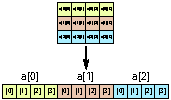
\includegraphics[width=0.5\textwidth]{2dto1d.pdf}
\end{center}\end{center} 
\begin{itemize}
\item \alert{Achtung: Diese manuelle Methode ist \uline{NICHT} langsamer als das was C intern macht!}
\item Ich bevorzuge diese Methode, da sie meiner Meinung nach \alert{einfacher
und flexibler} ist
\end{itemize}
\end{frame}

\begin{frame}[label={sec:org1a49f3f}]{Manuell --- Zeilenanfang ermitteln}
\begin{center}\begin{center}
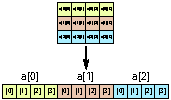
\includegraphics[width=0.5\textwidth]{2dto1d.pdf}
\end{center}\end{center} 
\begin{itemize}
\item Um auf ein Element in einer gewissen Zeile zuzugreifen müssen wir
also berechnen wo diese Zeile im Array anfängt. Wo die Zeile anfängt
hängt davon ab, wie lang eine Zeile ist (also die Anzahl an Spalten)
\begin{itemize}
\item \alert{Anfang der Zeile = Zeilennummer \texttimes{} Anzahl an Spalten}
\item z.B. Anfang der Zeile 2 = \(2 \times 4 = 8\)
\end{itemize}
\end{itemize}
\end{frame}
\begin{frame}[label={sec:org6071735}]{Manuell --- Berücksichtigen der Spalte}
\begin{center}\begin{center}
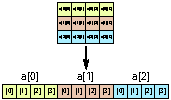
\includegraphics[width=0.5\textwidth]{2dto1d.pdf}
\end{center}\end{center} 
\begin{itemize}
\item Wir wissen jetzt an welcher Position eine Zeile anfängt. Wenn wir
ein Element in dieser Zeile in einer bestimmten Spalte wollen
addieren wir zum Zeilenanfang die Spaltennummer
\begin{itemize}
\item \alert{Position von Element = Zeilennummer \texttimes{} Anzahl an Spalten + Spaltennummer}
\item z.B. Position von Element in Zeile 1 und Spalte 2 = \(1 \times 4 + 2 = 6\)
\end{itemize}
\end{itemize}
\end{frame}
\begin{frame}[label={sec:orgabda218},fragile]{Manuell --- Beispiel}
 \begin{block}{Beispiel}
\begin{minted}[fontsize=\scriptsize,numberblanklines=false]{c}
#include <stdio.h>

int main() {
  int rows = 3;
  int cols = 4;
  int a[12] = {1, 2, 3, 4, 5, 6, 7, 8, 9, 10, 11, 12};

  for (int row = 0; row < 3; row++) {
    for (int col = 0; col < 4; col++)
      printf("%d\t", a[row * cols + col]);
    printf("\n");
  }
}
\end{minted}
\end{block}
\end{frame}
\begin{frame}[label={sec:orgc956e6e},fragile]{Manuell --- Beispiel --- Übergabe an Funktionen}
 \begin{block}{Beispiel}
\begin{minted}[fontsize=\scriptsize,numberblanklines=false]{c}
#include <stdio.h>

void print_matrix(int *arr, int rows, int cols) {
  for (int row = 0; row < rows; row++) {
    for (int col = 0; col < cols; col++)
      printf("%d\t", arr[row * cols + col]);
    printf("\n");
  }
}

int main() {
  int a[3][4] = {{1, 2, 3, 4}, {5, 6, 7, 8}, {9, 10, 11, 12}};
  print_matrix(a, 3, 4);
}
\end{minted}
\end{block}
\end{frame}

\begin{frame}[label={sec:orgfbc042b}]{Dynamische Speicherverwaltung}
\begin{itemize}
\item Man kann mittels dynamischer Speicherverwaltung mehrdimensionale
Arrays erzeugen die sich verhalten wie die von C intern
unterstützten. Das ist aber relativ umständlich und kompliziert
\item Meine Empfehlung: \alert{Verwenden der manuellen Methode}
\end{itemize}
\end{frame}
\begin{frame}[label={sec:orgbcfecf0}]{Gemeinsames Beispiel}
Wir wollen in einem 2D Array speichern was an einer bestimmten
Position als Hintergrund gezeichnet werden soll
\begin{center}\begin{center}
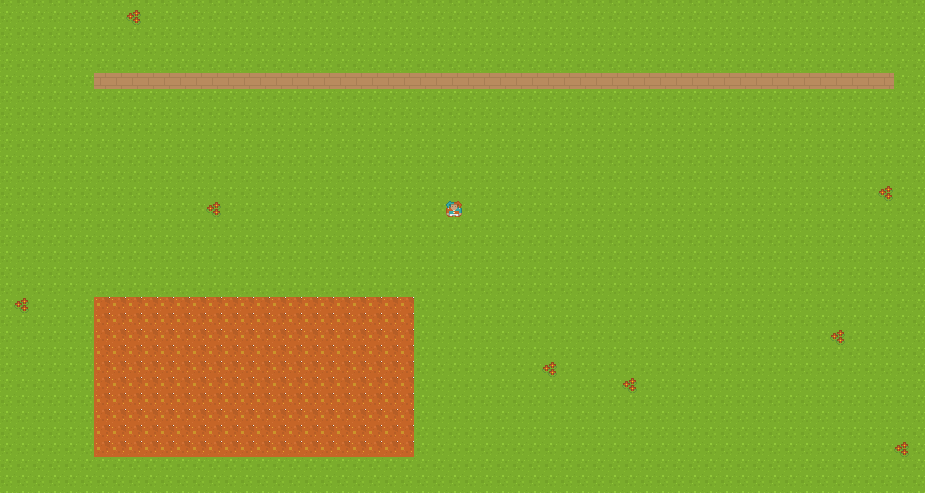
\includegraphics[width=.9\linewidth]{data/00/1df613-db63-4675-993c-1159913a0378/screenshot-20200507-214418.png}
\end{center}\end{center}
\end{frame}
\begin{frame}[label={sec:orge1c6a23},fragile]{Übung}
 \begin{itemize}
\item Erweitern Sie das vorherige Beispiel so, dass Sie in einem zweiten
2D Array speichern welche Felder begehbar sind und welche nicht
\item Übergeben Sie dieses Array an die Bewegungsfunktionen ({\color{solarizedYellow}\texttt{move\_left}},
{\color{solarizedYellow}\texttt{move\_right}}, {\color{solarizedYellow}\texttt{move\_up}}, {\color{solarizedYellow}\texttt{move\_down}}) und verhindern Sie in diesen,
dass unsere Spielfigur Felder betreten kann welche als nicht
begehbar markiert sind.
\item Machen Sie damit unsere gezeichnete Mauer unpassierbar
\end{itemize}
\begin{center}\begin{center}
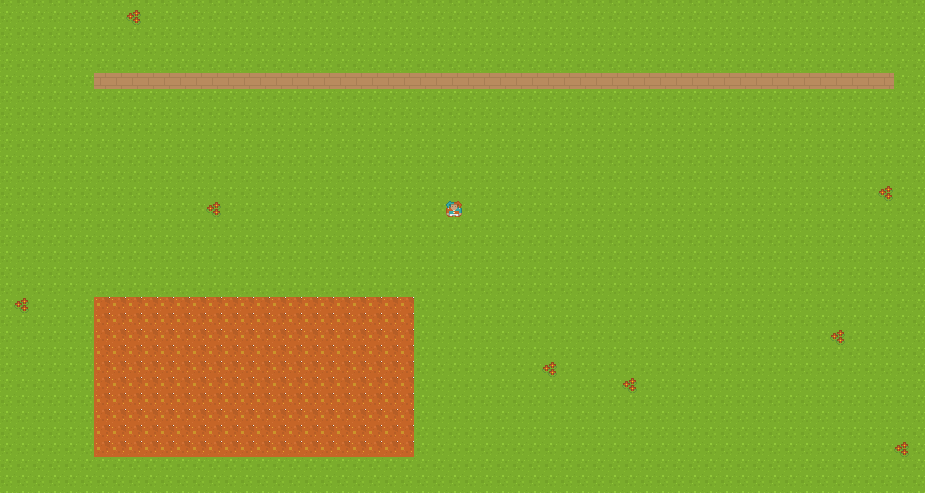
\includegraphics[width=0.6\textwidth]{data/00/1df613-db63-4675-993c-1159913a0378/screenshot-20200507-214418.png}
\end{center}\end{center}
\end{frame}
\end{document}